\documentclass[twoside]{book}

% Packages required by doxygen
\usepackage{fixltx2e}
\usepackage{calc}
\usepackage{doxygen}
\usepackage[export]{adjustbox} % also loads graphicx
\usepackage{graphicx}
\usepackage[utf8]{inputenc}
\usepackage{makeidx}
\usepackage{multicol}
\usepackage{multirow}
\PassOptionsToPackage{warn}{textcomp}
\usepackage{textcomp}
\usepackage[nointegrals]{wasysym}
\usepackage[table]{xcolor}

% Font selection
\usepackage[T1]{fontenc}
\usepackage[scaled=.90]{helvet}
\usepackage{courier}
\usepackage{amssymb}
\usepackage{sectsty}
\renewcommand{\familydefault}{\sfdefault}
\allsectionsfont{%
  \fontseries{bc}\selectfont%
  \color{darkgray}%
}
\renewcommand{\DoxyLabelFont}{%
  \fontseries{bc}\selectfont%
  \color{darkgray}%
}
\newcommand{\+}{\discretionary{\mbox{\scriptsize$\hookleftarrow$}}{}{}}

% Page & text layout
\usepackage{geometry}
\geometry{%
  a4paper,%
  top=2.5cm,%
  bottom=2.5cm,%
  left=2.5cm,%
  right=2.5cm%
}
\tolerance=750
\hfuzz=15pt
\hbadness=750
\setlength{\emergencystretch}{15pt}
\setlength{\parindent}{0cm}
\setlength{\parskip}{3ex plus 2ex minus 2ex}
\makeatletter
\renewcommand{\paragraph}{%
  \@startsection{paragraph}{4}{0ex}{-1.0ex}{1.0ex}{%
    \normalfont\normalsize\bfseries\SS@parafont%
  }%
}
\renewcommand{\subparagraph}{%
  \@startsection{subparagraph}{5}{0ex}{-1.0ex}{1.0ex}{%
    \normalfont\normalsize\bfseries\SS@subparafont%
  }%
}
\makeatother

% Headers & footers
\usepackage{fancyhdr}
\pagestyle{fancyplain}
\fancyhead[LE]{\fancyplain{}{\bfseries\thepage}}
\fancyhead[CE]{\fancyplain{}{}}
\fancyhead[RE]{\fancyplain{}{\bfseries\leftmark}}
\fancyhead[LO]{\fancyplain{}{\bfseries\rightmark}}
\fancyhead[CO]{\fancyplain{}{}}
\fancyhead[RO]{\fancyplain{}{\bfseries\thepage}}
\fancyfoot[LE]{\fancyplain{}{}}
\fancyfoot[CE]{\fancyplain{}{}}
\fancyfoot[RE]{\fancyplain{}{\bfseries\scriptsize Generated by Doxygen }}
\fancyfoot[LO]{\fancyplain{}{\bfseries\scriptsize Generated by Doxygen }}
\fancyfoot[CO]{\fancyplain{}{}}
\fancyfoot[RO]{\fancyplain{}{}}
\renewcommand{\footrulewidth}{0.4pt}
\renewcommand{\chaptermark}[1]{%
  \markboth{#1}{}%
}
\renewcommand{\sectionmark}[1]{%
  \markright{\thesection\ #1}%
}

% Indices & bibliography
\usepackage{natbib}
\usepackage[titles]{tocloft}
\setcounter{tocdepth}{3}
\setcounter{secnumdepth}{5}
\makeindex

% Hyperlinks (required, but should be loaded last)
\usepackage{ifpdf}
\ifpdf
  \usepackage[pdftex,pagebackref=true]{hyperref}
\else
  \usepackage[ps2pdf,pagebackref=true]{hyperref}
\fi
\hypersetup{%
  colorlinks=true,%
  linkcolor=blue,%
  citecolor=blue,%
  unicode%
}

% Custom commands
\newcommand{\clearemptydoublepage}{%
  \newpage{\pagestyle{empty}\cleardoublepage}%
}

\usepackage{caption}
\captionsetup{labelsep=space,justification=centering,font={bf},singlelinecheck=off,skip=4pt,position=top}

%===== C O N T E N T S =====

\begin{document}

% Titlepage & ToC
\hypersetup{pageanchor=false,
             bookmarksnumbered=true,
             pdfencoding=unicode
            }
\pagenumbering{roman}
\begin{titlepage}
\vspace*{7cm}
\begin{center}%
{\Large Vinte Perguntas }\\
\vspace*{1cm}
{\large Generated by Doxygen 1.8.11}\\
\end{center}
\end{titlepage}
\clearemptydoublepage
\tableofcontents
\clearemptydoublepage
\pagenumbering{arabic}
\hypersetup{pageanchor=true}

%--- Begin generated contents ---
\chapter{Class Index}
\section{Class List}
Here are the classes, structs, unions and interfaces with brief descriptions\+:\begin{DoxyCompactList}
\item\contentsline{section}{\hyperlink{structnode}{node} }{\pageref{structnode}}{}
\end{DoxyCompactList}

\chapter{File Index}
\section{File List}
Here is a list of all files with brief descriptions\+:\begin{DoxyCompactList}
\item\contentsline{section}{\hyperlink{funcoes_8c}{funcoes.\+c} }{\pageref{funcoes_8c}}{}
\item\contentsline{section}{\hyperlink{main_8c}{main.\+c} }{\pageref{main_8c}}{}
\end{DoxyCompactList}

\chapter{Class Documentation}
\hypertarget{structnode}{}\section{node Struct Reference}
\label{structnode}\index{node@{node}}


Collaboration diagram for node\+:\nopagebreak
\begin{figure}[H]
\begin{center}
\leavevmode
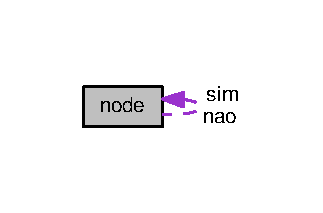
\includegraphics[width=155pt]{structnode__coll__graph}
\end{center}
\end{figure}
\subsection*{Public Attributes}
\begin{DoxyCompactItemize}
\item 
int \hyperlink{structnode_aae328428a1fb362e7e7aca4b3ad67470}{valor}
\item 
char $\ast$ \hyperlink{structnode_a55a6556b4365a179d03ca038fad7530c}{pergunta}
\item 
struct \hyperlink{structnode}{node} $\ast$ \hyperlink{structnode_a7f67cb5c3c6ed869d7e9a204af095135}{sim}
\item 
struct \hyperlink{structnode}{node} $\ast$ \hyperlink{structnode_a295980223d27becf8725335bbd5d1c61}{nao}
\end{DoxyCompactItemize}


\subsection{Member Data Documentation}
\index{node@{node}!nao@{nao}}
\index{nao@{nao}!node@{node}}
\subsubsection[{\texorpdfstring{nao}{nao}}]{\setlength{\rightskip}{0pt plus 5cm}struct {\bf node}$\ast$ node\+::nao}\hypertarget{structnode_a295980223d27becf8725335bbd5d1c61}{}\label{structnode_a295980223d27becf8725335bbd5d1c61}
\index{node@{node}!pergunta@{pergunta}}
\index{pergunta@{pergunta}!node@{node}}
\subsubsection[{\texorpdfstring{pergunta}{pergunta}}]{\setlength{\rightskip}{0pt plus 5cm}char$\ast$ node\+::pergunta}\hypertarget{structnode_a55a6556b4365a179d03ca038fad7530c}{}\label{structnode_a55a6556b4365a179d03ca038fad7530c}
\index{node@{node}!sim@{sim}}
\index{sim@{sim}!node@{node}}
\subsubsection[{\texorpdfstring{sim}{sim}}]{\setlength{\rightskip}{0pt plus 5cm}struct {\bf node}$\ast$ node\+::sim}\hypertarget{structnode_a7f67cb5c3c6ed869d7e9a204af095135}{}\label{structnode_a7f67cb5c3c6ed869d7e9a204af095135}
\index{node@{node}!valor@{valor}}
\index{valor@{valor}!node@{node}}
\subsubsection[{\texorpdfstring{valor}{valor}}]{\setlength{\rightskip}{0pt plus 5cm}int node\+::valor}\hypertarget{structnode_aae328428a1fb362e7e7aca4b3ad67470}{}\label{structnode_aae328428a1fb362e7e7aca4b3ad67470}


The documentation for this struct was generated from the following file\+:\begin{DoxyCompactItemize}
\item 
\hyperlink{funcoes_8c}{funcoes.\+c}\end{DoxyCompactItemize}

\chapter{File Documentation}
\hypertarget{arvore_8txt}{}\section{arvore.\+txt File Reference}
\label{arvore_8txt}\index{arvore.\+txt@{arvore.\+txt}}

\hypertarget{funcoes_8c}{}\section{funcoes.\+c File Reference}
\label{funcoes_8c}\index{funcoes.\+c@{funcoes.\+c}}
{\ttfamily \#include $<$stdio.\+h$>$}\\*
{\ttfamily \#include $<$stdlib.\+h$>$}\\*
{\ttfamily \#include $<$string.\+h$>$}\\*
{\ttfamily \#include $<$unistd.\+h$>$}\\*
Include dependency graph for funcoes.\+c\+:\nopagebreak
\begin{figure}[H]
\begin{center}
\leavevmode
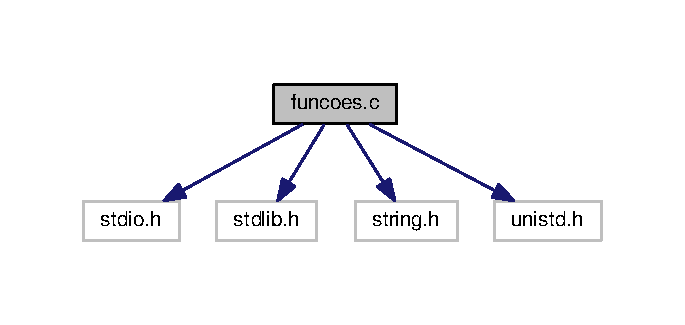
\includegraphics[width=329pt]{funcoes_8c__incl}
\end{center}
\end{figure}
\subsection*{Classes}
\begin{DoxyCompactItemize}
\item 
struct \hyperlink{structnode}{node}
\end{DoxyCompactItemize}
\subsection*{Typedefs}
\begin{DoxyCompactItemize}
\item 
typedef struct \hyperlink{structnode}{node} \hyperlink{funcoes_8c_a194aa098fccd2d4ab0e67b349d0db930}{tree}
\end{DoxyCompactItemize}
\subsection*{Functions}
\begin{DoxyCompactItemize}
\item 
void \hyperlink{funcoes_8c_a9d7e8af417b6d543da691e9c0e2f6f9f}{clear\+Screen} ()
\item 
\hyperlink{funcoes_8c_a194aa098fccd2d4ab0e67b349d0db930}{tree} $\ast$ \hyperlink{funcoes_8c_a8a1d4d10337fa6080896c2a329d696d1}{new\+Node} (char $\ast$pergunta, int valor)
\item 
\hyperlink{funcoes_8c_a194aa098fccd2d4ab0e67b349d0db930}{tree} $\ast$ \hyperlink{funcoes_8c_a121cf062cb8d021f0f0aec61e719ba49}{delete\+Tree} (\hyperlink{funcoes_8c_a194aa098fccd2d4ab0e67b349d0db930}{tree} $\ast$del)
\item 
void \hyperlink{funcoes_8c_aa893184ff708158578bacb94ac2ac41e}{save\+Tree} (\hyperlink{funcoes_8c_a194aa098fccd2d4ab0e67b349d0db930}{tree} $\ast$save, F\+I\+LE $\ast$fp)
\item 
\hyperlink{funcoes_8c_a194aa098fccd2d4ab0e67b349d0db930}{tree} $\ast$ \hyperlink{funcoes_8c_a6b9025f47b1391cb6e7d9252273b8d00}{load\+Tree} (\hyperlink{funcoes_8c_a194aa098fccd2d4ab0e67b349d0db930}{tree} $\ast$$\ast$save, \hyperlink{funcoes_8c_a194aa098fccd2d4ab0e67b349d0db930}{tree} $\ast$$\ast$anterior, F\+I\+LE $\ast$fp, int posicao, int lado)
\item 
\hyperlink{funcoes_8c_a194aa098fccd2d4ab0e67b349d0db930}{tree} $\ast$ \hyperlink{funcoes_8c_a6b9d8c00654348cd9683bdd0299df851}{create\+Game} (\hyperlink{funcoes_8c_a194aa098fccd2d4ab0e67b349d0db930}{tree} $\ast$$\ast$atual, \hyperlink{funcoes_8c_a194aa098fccd2d4ab0e67b349d0db930}{tree} $\ast$$\ast$anterior, int altura, int $\ast$deleted\+\_\+position, F\+I\+LE $\ast$fp)
\item 
void \hyperlink{funcoes_8c_a1e840c01b998f6885081f7bbc4d4fcd5}{play\+Game} (\hyperlink{funcoes_8c_a194aa098fccd2d4ab0e67b349d0db930}{tree} $\ast$$\ast$atual, int altura)
\item 
\hyperlink{funcoes_8c_a194aa098fccd2d4ab0e67b349d0db930}{tree} $\ast$ \hyperlink{funcoes_8c_a6178b4c4d1e451e109557caa1d156412}{choose\+Menu} (\hyperlink{funcoes_8c_a194aa098fccd2d4ab0e67b349d0db930}{tree} $\ast$load, int $\ast$selecao)
\end{DoxyCompactItemize}


\subsection{Typedef Documentation}
\index{funcoes.\+c@{funcoes.\+c}!tree@{tree}}
\index{tree@{tree}!funcoes.\+c@{funcoes.\+c}}
\subsubsection[{\texorpdfstring{tree}{tree}}]{\setlength{\rightskip}{0pt plus 5cm}typedef struct {\bf node}  {\bf tree}}\hypertarget{funcoes_8c_a194aa098fccd2d4ab0e67b349d0db930}{}\label{funcoes_8c_a194aa098fccd2d4ab0e67b349d0db930}


\subsection{Function Documentation}
\index{funcoes.\+c@{funcoes.\+c}!choose\+Menu@{choose\+Menu}}
\index{choose\+Menu@{choose\+Menu}!funcoes.\+c@{funcoes.\+c}}
\subsubsection[{\texorpdfstring{choose\+Menu(tree $\ast$load, int $\ast$selecao)}{chooseMenu(tree *load, int *selecao)}}]{\setlength{\rightskip}{0pt plus 5cm}{\bf tree}$\ast$ choose\+Menu (
\begin{DoxyParamCaption}
\item[{{\bf tree} $\ast$}]{load, }
\item[{int $\ast$}]{selecao}
\end{DoxyParamCaption}
)}\hypertarget{funcoes_8c_a6178b4c4d1e451e109557caa1d156412}{}\label{funcoes_8c_a6178b4c4d1e451e109557caa1d156412}
\index{funcoes.\+c@{funcoes.\+c}!clear\+Screen@{clear\+Screen}}
\index{clear\+Screen@{clear\+Screen}!funcoes.\+c@{funcoes.\+c}}
\subsubsection[{\texorpdfstring{clear\+Screen()}{clearScreen()}}]{\setlength{\rightskip}{0pt plus 5cm}void clear\+Screen (
\begin{DoxyParamCaption}
{}
\end{DoxyParamCaption}
)}\hypertarget{funcoes_8c_a9d7e8af417b6d543da691e9c0e2f6f9f}{}\label{funcoes_8c_a9d7e8af417b6d543da691e9c0e2f6f9f}
\index{funcoes.\+c@{funcoes.\+c}!create\+Game@{create\+Game}}
\index{create\+Game@{create\+Game}!funcoes.\+c@{funcoes.\+c}}
\subsubsection[{\texorpdfstring{create\+Game(tree $\ast$$\ast$atual, tree $\ast$$\ast$anterior, int altura, int $\ast$deleted\+\_\+position, F\+I\+L\+E $\ast$fp)}{createGame(tree **atual, tree **anterior, int altura, int *deleted_position, FILE *fp)}}]{\setlength{\rightskip}{0pt plus 5cm}{\bf tree}$\ast$ create\+Game (
\begin{DoxyParamCaption}
\item[{{\bf tree} $\ast$$\ast$}]{atual, }
\item[{{\bf tree} $\ast$$\ast$}]{anterior, }
\item[{int}]{altura, }
\item[{int $\ast$}]{deleted\+\_\+position, }
\item[{F\+I\+LE $\ast$}]{fp}
\end{DoxyParamCaption}
)}\hypertarget{funcoes_8c_a6b9d8c00654348cd9683bdd0299df851}{}\label{funcoes_8c_a6b9d8c00654348cd9683bdd0299df851}
\index{funcoes.\+c@{funcoes.\+c}!delete\+Tree@{delete\+Tree}}
\index{delete\+Tree@{delete\+Tree}!funcoes.\+c@{funcoes.\+c}}
\subsubsection[{\texorpdfstring{delete\+Tree(tree $\ast$del)}{deleteTree(tree *del)}}]{\setlength{\rightskip}{0pt plus 5cm}{\bf tree}$\ast$ delete\+Tree (
\begin{DoxyParamCaption}
\item[{{\bf tree} $\ast$}]{del}
\end{DoxyParamCaption}
)}\hypertarget{funcoes_8c_a121cf062cb8d021f0f0aec61e719ba49}{}\label{funcoes_8c_a121cf062cb8d021f0f0aec61e719ba49}
\index{funcoes.\+c@{funcoes.\+c}!load\+Tree@{load\+Tree}}
\index{load\+Tree@{load\+Tree}!funcoes.\+c@{funcoes.\+c}}
\subsubsection[{\texorpdfstring{load\+Tree(tree $\ast$$\ast$save, tree $\ast$$\ast$anterior, F\+I\+L\+E $\ast$fp, int posicao, int lado)}{loadTree(tree **save, tree **anterior, FILE *fp, int posicao, int lado)}}]{\setlength{\rightskip}{0pt plus 5cm}{\bf tree}$\ast$ load\+Tree (
\begin{DoxyParamCaption}
\item[{{\bf tree} $\ast$$\ast$}]{save, }
\item[{{\bf tree} $\ast$$\ast$}]{anterior, }
\item[{F\+I\+LE $\ast$}]{fp, }
\item[{int}]{posicao, }
\item[{int}]{lado}
\end{DoxyParamCaption}
)}\hypertarget{funcoes_8c_a6b9025f47b1391cb6e7d9252273b8d00}{}\label{funcoes_8c_a6b9025f47b1391cb6e7d9252273b8d00}
\index{funcoes.\+c@{funcoes.\+c}!new\+Node@{new\+Node}}
\index{new\+Node@{new\+Node}!funcoes.\+c@{funcoes.\+c}}
\subsubsection[{\texorpdfstring{new\+Node(char $\ast$pergunta, int valor)}{newNode(char *pergunta, int valor)}}]{\setlength{\rightskip}{0pt plus 5cm}{\bf tree}$\ast$ new\+Node (
\begin{DoxyParamCaption}
\item[{char $\ast$}]{pergunta, }
\item[{int}]{valor}
\end{DoxyParamCaption}
)}\hypertarget{funcoes_8c_a8a1d4d10337fa6080896c2a329d696d1}{}\label{funcoes_8c_a8a1d4d10337fa6080896c2a329d696d1}
\index{funcoes.\+c@{funcoes.\+c}!play\+Game@{play\+Game}}
\index{play\+Game@{play\+Game}!funcoes.\+c@{funcoes.\+c}}
\subsubsection[{\texorpdfstring{play\+Game(tree $\ast$$\ast$atual, int altura)}{playGame(tree **atual, int altura)}}]{\setlength{\rightskip}{0pt plus 5cm}void play\+Game (
\begin{DoxyParamCaption}
\item[{{\bf tree} $\ast$$\ast$}]{atual, }
\item[{int}]{altura}
\end{DoxyParamCaption}
)}\hypertarget{funcoes_8c_a1e840c01b998f6885081f7bbc4d4fcd5}{}\label{funcoes_8c_a1e840c01b998f6885081f7bbc4d4fcd5}
\index{funcoes.\+c@{funcoes.\+c}!save\+Tree@{save\+Tree}}
\index{save\+Tree@{save\+Tree}!funcoes.\+c@{funcoes.\+c}}
\subsubsection[{\texorpdfstring{save\+Tree(tree $\ast$save, F\+I\+L\+E $\ast$fp)}{saveTree(tree *save, FILE *fp)}}]{\setlength{\rightskip}{0pt plus 5cm}void save\+Tree (
\begin{DoxyParamCaption}
\item[{{\bf tree} $\ast$}]{save, }
\item[{F\+I\+LE $\ast$}]{fp}
\end{DoxyParamCaption}
)}\hypertarget{funcoes_8c_aa893184ff708158578bacb94ac2ac41e}{}\label{funcoes_8c_aa893184ff708158578bacb94ac2ac41e}

\hypertarget{main_8c}{}\section{main.\+c File Reference}
\label{main_8c}\index{main.\+c@{main.\+c}}
{\ttfamily \#include $<$stdio.\+h$>$}\\*
{\ttfamily \#include $<$stdlib.\+h$>$}\\*
{\ttfamily \#include $<$string.\+h$>$}\\*
{\ttfamily \#include $<$unistd.\+h$>$}\\*
{\ttfamily \#include $<$funcoes.\+h$>$}\\*
Include dependency graph for main.\+c\+:\nopagebreak
\begin{figure}[H]
\begin{center}
\leavevmode
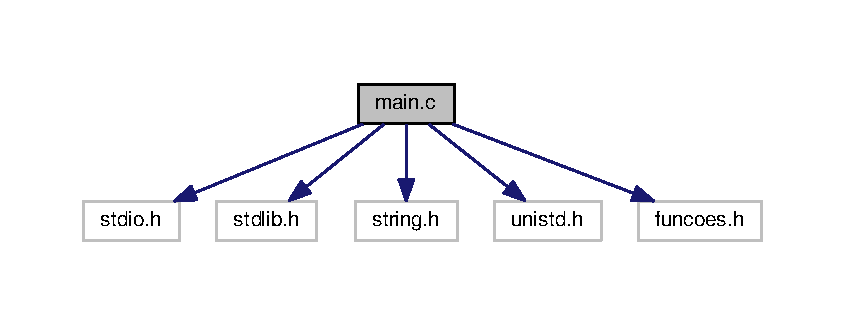
\includegraphics[width=350pt]{main_8c__incl}
\end{center}
\end{figure}
\subsection*{Functions}
\begin{DoxyCompactItemize}
\item 
int \hyperlink{main_8c_ae66f6b31b5ad750f1fe042a706a4e3d4}{main} ()
\end{DoxyCompactItemize}


\subsection{Function Documentation}
\index{main.\+c@{main.\+c}!main@{main}}
\index{main@{main}!main.\+c@{main.\+c}}
\subsubsection[{\texorpdfstring{main()}{main()}}]{\setlength{\rightskip}{0pt plus 5cm}int main (
\begin{DoxyParamCaption}
{}
\end{DoxyParamCaption}
)}\hypertarget{main_8c_ae66f6b31b5ad750f1fe042a706a4e3d4}{}\label{main_8c_ae66f6b31b5ad750f1fe042a706a4e3d4}

%--- End generated contents ---

% Index
\backmatter
\newpage
\phantomsection
\clearemptydoublepage
\addcontentsline{toc}{chapter}{Index}
\printindex

\end{document}
